\documentclass[12pt]{article}
\usepackage[a4paper, total={5.7in, 9in}]{geometry}
\usepackage{url}
\usepackage{hyperref}
\usepackage{graphicx}
\usepackage{booktabs}
\usepackage{amsmath}
\usepackage{listings}
\usepackage{xcolor}
\usepackage{tikz}
\usetikzlibrary{shapes, arrows.meta, positioning, fit}

\lstset{
  basicstyle=\ttfamily\small,
  breaklines=true,
  frame=single,
  backgroundcolor=\color{gray!10},
  keywordstyle=\color{blue},
  commentstyle=\color{green!50!black},
  stringstyle=\color{red!70!black},
  showstringspaces=false
}

\begin{document}
\title{BDI Multi-Agent System for Lung Nodule Evidence Extraction from Chest X-ray Reports}
\author{Sepehr Khodadadi Hosseinabadi\\
{\em 6660699@studenti.unige.it}}
\maketitle

% =============================================================================
% PROPOSAL PAGE (not counted)
% =============================================================================
\section{Details of the Proposal}
\label{sec:yourProposal}

\subsection{Full Specification of the Proposal}
\label{subsec:specification}

I will build a complete BDI multi-agent system in which all agents are BDI agents that interoperate by message passing, while only the CV Radiologist uses a pre-trained model and the NLP is implemented by me. The use case is lung nodule evidence extraction from chest X-ray radiology reports, paired with the corresponding X-ray images from the IU/Open-I chest X-ray collection (English reports). The dataset contains around 7,470 images and reports. I will use an NLP-based pre-filter to select 30--50 image--report pairs whose reports mention lung nodules, and I will annotate them for evaluation of my NLP outputs (entities + attributes + negation/uncertainty).



\subsection{The Kind of the Proposal}
\label{subsec:kind}

My proposal consists of a creative project.

\subsection{The Range of Points/Difficulty of the Proposal}
\label{subsec:points}

The degree of difficulty for this project is hard.

\pagebreak

% =============================================================================
% INTRODUCTION
% =============================================================================
\section{Introduction}
\label{sec:intro}

Lung cancer is the leading cause of cancer-related death worldwide, and early detection of pulmonary nodules is critical for improving patient outcomes. Radiology reports offer a rich source of structured and unstructured clinical information, yet extracting actionable evidence from free-text\footnote{free-text reports are reports that are not structured in a way that can be easily processed by a computer} reports remains a challenging NLP task. Simultaneously, medical imaging with deep learning has shown promise for automated nodule detection, but individual models vary in their sensitivity and specificity.

This project addresses the problem of \emph{lung nodule evidence extraction and fusion} by combining three complementary AI paradigms within a multi-agent architecture:

\begin{enumerate}
    \item \textbf{Natural Language Processing (NLP):} Extracting structured nodule attributes (size, location, texture, descriptors), detecting mentions, and determining negation/uncertainty status from free-text radiology reports.
    \item \textbf{Computer Vision (CV):} Obtaining nodule suspicion scores from chest X-ray images using the \texttt{TorchXRayVision} library~\cite{cohen2022xrv}, leveraging models pretrained on massive chest X-ray datasets.
    \item \textbf{Symbolic Reasoning:} Combining the outputs of multiple NLP and CV agents using first-order logic rules encoded in Prolog, implementing weighted consensus, conflict detection, and clinical recommendation generation.
\end{enumerate}

The system is organized as a \emph{Belief--Desire--Intention (BDI) multi-agent system}~\cite{rao2005bdi}, where each agent maintains beliefs about the world, desires (goals) it aims to achieve, and intentions (plans) it commits to executing. This architecture is particularly well-suited for medical decision support because it mirrors the clinical workflow: independent specialists (radiologists, pathologists) generate findings that are synthesized by a coordinating physician (oncologist) into a final recommendation.

\subsection{Clinical Motivation}
\label{subsec:clinical-motivation}

In standard clinical practice, the workflow for lung nodule management follows a hub-and-spoke model: radiologists analyze images and produce reports, pathologists analyze tissue or textual evidence, and the treating oncologist synthesizes all findings into a treatment decision~\cite{pillay2016mdt}. Direct communication between radiologists and pathologists is uncommon in routine practice---they work independently and send reports to the treating physician. This clinically accurate architecture is reflected in our system design, where all agents report to the central Oncologist agent rather than communicating peer-to-peer.

\subsection{Dataset}
\label{subsec:dataset}

The system operates on the IU/Open-I Indiana University Chest X-ray Collection~\cite{demsar2005openi}, which contains approximately 7,470 chest X-ray images paired with free-text radiology reports. Each report is structured in XML format with fields for findings, impressions, and indications. From this collection, we apply an NLP-based pre-filter to select 30--50 cases whose reports explicitly mention pulmonary nodules, forming the evaluation subset. This subset size is consistent with prior clinical NLP validation studies---for instance, Chapman et al.\ used 42 reports for NegEx evaluation~\cite{chapman2001negex}.

\subsection{Contributions}
\label{subsec:contributions}

The main contributions of this project are:

\begin{enumerate}
    \item A complete BDI multi-agent system with 7 agent instances across 3 agent types, communicating via FIPA-compliant message passing.
    \item A custom NLP pipeline for lung nodule evidence extraction implementing: report section splitting with section weighting, entity and attribute extraction, measurement normalization, and NegEx-style negation and uncertainty detection.
    \item A Prolog-based consensus mechanism that performs weighted voting, disagreement detection, conflict resolution, and explanation generation.
    \item An end-to-end evaluation on real clinical reports with manually annotated entity-level ground truth.
\end{enumerate}


% =============================================================================
% BACKGROUND
% =============================================================================
\section{Background and Related Work}
\label{sec:background}

\subsection{NLP in Radiology}
\label{subsec:nlp-radiology}

Pons et al.~\cite{pons2016nlpradiology} present a systematic review of NLP applications in radiology, describing a canonical pipeline consisting of: (i) report section splitting (e.g., separating Findings from Impression); (ii) tokenization and normalization (handling abbreviations and standardizing measurements); (iii) syntactic and semantic processing; and (iv) application-specific extraction. They emphasize that \emph{negation detection} is essential for clinical NLP, since a large proportion of medical concepts in radiology reports appear in negated contexts (e.g., ``no evidence of nodule''). Our NLP pipeline follows this structure, with each stage implemented across three specialized Pathologist agents.

\subsection{Negation and Uncertainty Detection}
\label{subsec:negation}

Chapman et al.~\cite{chapman2001negex} introduced NegEx, a simple algorithm for identifying negated findings in clinical text. The algorithm operates by: (1) detecting \emph{trigger phrases} (e.g., ``no'', ``without'', ``denies'', ``ruled out''); (2) defining a forward or backward \emph{scope window} (typically 5--6 words); and (3) marking any medical entity within that scope as negated. Harkema et al.~\cite{harkema2009context} extended this approach with ConText, adding support for experiencer identification and temporal status.

For uncertainty detection, the CheXpert labeler~\cite{irvin2019chexpert} demonstrated that rule-based approaches can effectively classify radiology report mentions as positive, negative, or uncertain using trigger words such as ``possible'', ``cannot exclude'', ``may represent'', and ``suggestive of''. While CheXpert targets 14 chest X-ray observations, our project applies the same principles to the narrower task of nodule-specific attribute extraction.

\subsection{BDI Multi-Agent Systems}
\label{subsec:bdi}

The Belief--Desire--Intention (BDI) architecture~\cite{rao2005bdi} models rational agents that maintain: \emph{beliefs} (information about the environment), \emph{desires} (goals to achieve), and \emph{intentions} (committed plans). This architecture is implemented using the SPADE-BDI framework~\cite{spadebdi2023}, which uses AgentSpeak(L) plans triggered by belief changes and provides FIPA-compliant inter-agent messaging. In our implementation, `spade\_main.py` serves as the entry point, initializing specialized BDI agents that execute strict AgentSpeak logic defined in `.asl` files.

\subsection{Medical Decision Standards}
\label{subsec:medical-standards}

The Oncologist agent's reasoning layer encodes decision criteria grounded in two publicly documented medical standards:

\begin{itemize}
    \item \textbf{Lung-RADS v1.1}~\cite{acr2019lungrads}: The American College of Radiology's Lung Imaging Reporting and Data System defines categories from 1 (Negative) to 4X (Highly Suspicious) based on nodule size, texture, and morphological features. Although originally defined for low-dose CT screening, it provides a clear, codifiable mapping from nodule evidence to management recommendations.
    \item \textbf{TNM Staging (8th Edition)}~\cite{amin2017ajcc}: The AJCC TNM classification provides tumor staging based on tumor size (T), lymph node involvement (N), and distant metastasis (M). We reference the staging thresholds to ensure the rule base uses medically consistent vocabulary.
\end{itemize}


% =============================================================================
% SYSTEM ARCHITECTURE
% =============================================================================
\section{System Architecture}
\label{sec:architecture}

\subsection{Overview}
\label{subsec:arch-overview}

The system follows a hub-and-spoke architecture with three layers, mirroring the clinical workflow where independent specialists report to a coordinating physician:

\begin{figure}[h]
\centering
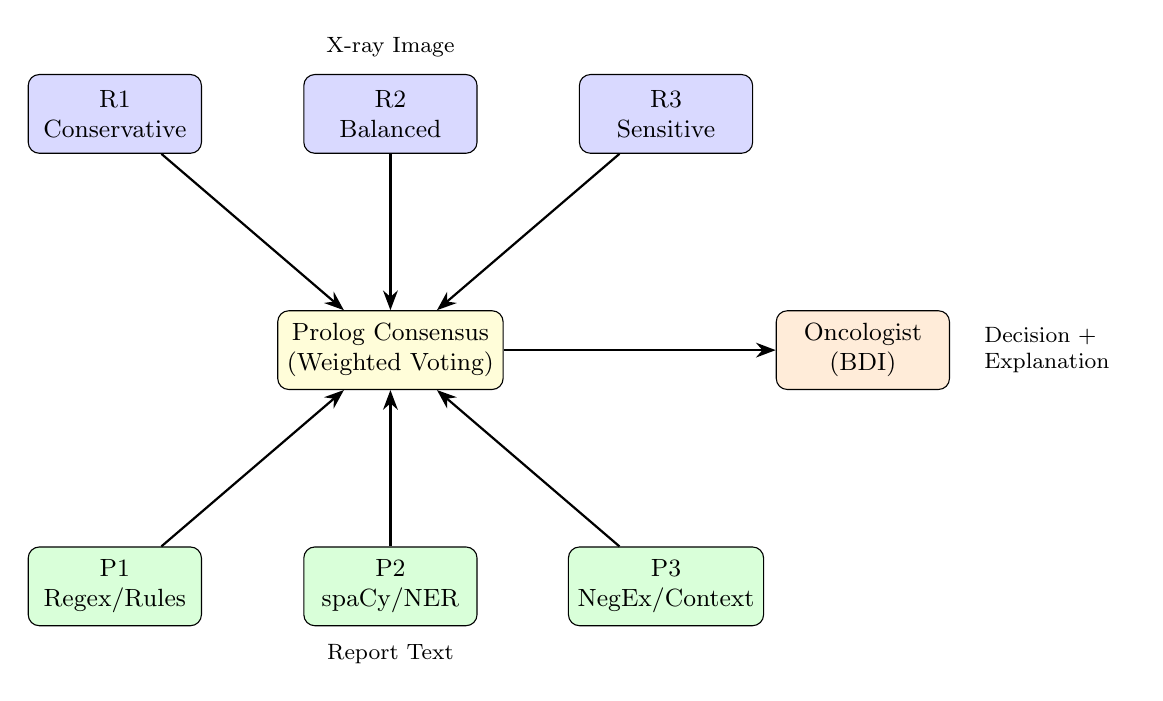
\begin{tikzpicture}[
    agent/.style={draw, rounded corners, minimum width=2.2cm, minimum height=1cm, align=center, font=\small},
    rads/.style={agent, fill=blue!15},
    paths/.style={agent, fill=green!15},
    onc/.style={agent, fill=orange!15},
    prolog/.style={agent, fill=yellow!15},
    arr/.style={-{Stealth[length=2.5mm]}, thick},
]
% Radiologists
\node[rads] (r1) at (-3.5, 3) {R1\\Conservative};
\node[rads] (r2) at (0, 3) {R2\\Balanced};
\node[rads] (r3) at (3.5, 3) {R3\\Sensitive};

% Pathologists
\node[paths] (p1) at (-3.5, -3) {P1\\Regex/Rules};
\node[paths] (p2) at (0, -3) {P2\\spaCy/NER};
\node[paths] (p3) at (3.5, -3) {P3\\NegEx/Context};

% Prolog
\node[prolog] (prolog) at (0, 0) {Prolog Consensus\\(Weighted Voting)};

% Oncologist
\node[onc] (onc) at (6, 0) {Oncologist\\(BDI)};

% Arrows
\draw[arr] (r1) -- (prolog);
\draw[arr] (r2) -- (prolog);
\draw[arr] (r3) -- (prolog);
\draw[arr] (p1) -- (prolog);
\draw[arr] (p2) -- (prolog);
\draw[arr] (p3) -- (prolog);
\draw[arr] (prolog) -- (onc);

% Input labels
\node[font=\footnotesize, above=0.1cm of r2] {X-ray Image};
\node[font=\footnotesize, below=0.1cm of p2] {Report Text};

% Output
\node[font=\footnotesize, right=0.1cm of onc] {\begin{tabular}{l}Decision +\\Explanation\end{tabular}};
\end{tikzpicture}
\caption{Multi-agent system architecture. Radiologist agents (R1--R3) process images; Pathologist agents (P1--P3) process report text. All findings are fused by the Prolog consensus engine, and the Oncologist produces the final decision with explanation.}
\label{fig:architecture}
\end{figure}

\subsection{Agent Descriptions}
\label{subsec:agents}

\subsubsection{Radiologist Agents (R1--R3)}
\label{subsubsec:radiologists}

The system deploys three distinct Radiologist agents to simulate clinical inter-reader variability. Each radiologist agent utilizes the \texttt{TorchXRayVision} library~\cite{cohen2022xrv}, employing a DenseNet-121 architecture~\cite{huang2020densenet} pretrained on a comprehensive aggregation of open chest X-ray datasets (including NIH, CheXpert, MIMIC-CXR, and PadChest). This ensures the features are domain-specific to thoracic pathology. The agents specifically monitor the model's output probability for the ``Nodule'' or ``Mass'' pathology classes. No additional CV training is performed; we rely on these robust frozen weights. The three agents differ in their functioning logic (using the model probability vs.\ heuristic feature-based fallbacks) and operating thresholds:

\begin{table}[h]
\centering
\begin{tabular}{llcl}
\toprule
\textbf{Agent} & \textbf{Style} & \textbf{Weight} & \textbf{Behavior} \\
\midrule
R1 & Conservative & 1.0 & High specificity, fewer false positives \\
R2 & Balanced     & 1.0 & Standard operating point \\
R3 & Sensitive    & 0.7 & High recall, fewer missed nodules \\
\bottomrule
\end{tabular}
\caption{Radiologist agent configurations.}
\label{tab:radiologists}
\end{table}

\subsubsection{Pathologist Agents (P1--P3)}
\label{subsubsec:pathologists}

The Pathologist agents are the main NLP contribution, with three active agents analyzing textual evidence. The 3rd agent (Pathologist-3), previously optional, is now fully enabled to handle negation and uncertainty. The term ``Pathologist'' is used metaphorically to represent agents that analyze textual evidence, analogous to how pathologists extract findings from specimens. Each agent implements a different NLP strategy:

\begin{table}[h]
\centering
\begin{tabular}{llcl}
\toprule
\textbf{Agent} & \textbf{Approach} & \textbf{Weight} & \textbf{Focus} \\
\midrule
P1 & Regex/Rules  & 0.8 & Robust patterns, section-based extraction \\
P2 & spaCy/NER    & 0.9 & Generalization, synonym handling \\
P3 & NegEx/Context & 0.9 & Negation and uncertainty detection \\
\bottomrule
\end{tabular}
\caption{Pathologist agent configurations.}
\label{tab:pathologists}
\end{table}

\subsubsection{Oncologist Agent}
\label{subsubsec:oncologist}

The Oncologist agent integrates all outputs using SWI-Prolog (accessed via PySwip~\cite{pyswip2023}). It implements:
\begin{itemize}
    \item Weighted voting: $P_\text{final} = \frac{\sum_{i} w_i \cdot c_i \cdot p_i}{\sum_{i} w_i \cdot c_i}$ where $w_i$ is the agent reliability weight, $c_i$ the reported confidence, and $p_i$ the malignancy probability.
    \item Conflict detection: disagreement is flagged when the standard deviation of agent probabilities exceeds 0.15.
    \item Resolution strategies: (1) trust CNN radiologists when NLP agrees; (2) use rule-based agent as tiebreaker; (3) conservative recommendation under strong disagreement.
    \item Explanation generation: a natural-language summary of which experts agreed/disagreed and which Prolog rule fired.
\end{itemize}


% =============================================================================
% NLP PIPELINE
% =============================================================================
\section{NLP Pipeline}
\label{sec:nlp}

The NLP pipeline follows the radiology NLP architecture described by Pons et al.~\cite{pons2016nlpradiology}. The pipeline is distributed across the three Pathologist agents, with each agent implementing complementary extraction strategies.

\subsection{Report Section Splitting}
\label{subsec:section-splitting}

Radiology reports in the Open-I collection follow a semi-structured format with standard section headers. The pipeline identifies and segments reports into sections:

\begin{lstlisting}[language=Python, caption={Section splitting with weighting.}]
SECTION_HEADERS = ["FINDINGS:", "IMPRESSION:", "INDICATION:",
                   "TECHNIQUE:", "COMPARISON:"]
SECTION_WEIGHTS = {"IMPRESSION": 1.5, "FINDINGS": 1.0,
                   "INDICATION": 0.5, "TECHNIQUE": 0.2}
\end{lstlisting}

The IMPRESSION section receives a higher weight (1.5$\times$) because it represents the radiologist's synthesis and clinical judgment, following standard clinical practice where impressions carry more diagnostic weight than descriptive findings.

\subsection{Tokenization and Normalization}
\label{subsec:tokenization}

Medical text requires specialized tokenization to handle:
\begin{itemize}
    \item \textbf{Abbreviations:} Common radiology abbreviations (RUL = right upper lobe, GGO = ground-glass opacity, CT, mm) are preserved during tokenization and expanded where needed via a lookup dictionary.
    \item \textbf{Measurement normalization:} Size mentions in different formats (``8 mm'', ``0.8 cm'', ``8mm'') are normalized to millimeters using regex patterns with unit conversion.
    \item \textbf{Hyphenated terms:} Medical compounds (``well-defined'', ``ground-glass'', ``part-solid'') are handled as single tokens.
\end{itemize}

When spaCy/scispaCy~\cite{neumann2019scispacy} is available (Pathologist-2), the pipeline uses its rule-based tokenizer with custom rules for medical text. Otherwise, regex-based tokenization is used (Pathologist-1).

\subsection{Nodule Mention Detection}
\label{subsec:mention-detection}

Nodule mentions are detected using a lexicon-based approach combined with patterns:

\begin{lstlisting}[language=Python, caption={Nodule mention lexicon.}]
NODULE_LEXICON = ["nodule", "nodular", "nodular opacity",
                  "mass", "lesion", "opacity", "tumor",
                  "pulmonary nodule", "lung nodule",
                  "solitary nodule", "spiculated mass"]
\end{lstlisting}

Pathologist-2 supplements this with scispaCy's biomedical NER model, which can recognize medical entities not present in the lexicon.

\subsection{Attribute Extraction}
\label{subsec:attribute-extraction}

Four categories of attributes are extracted:

\begin{enumerate}
    \item \textbf{Anatomical location:} Regex patterns for lobe references (``right upper lobe'', ``RUL''), positional terms (``subpleural'', ``perihilar''), and laterality.
    \item \textbf{Size mentions:} Multiple patterns capture formats including ``15 mm'', ``1.5 cm'', and dimensional notations (``15 $\times$ 12 mm''), with automatic unit normalization to millimeters.
    \item \textbf{Multiplicity:} Detection of plural nodule mentions (``multiple nodules'', ``bilateral'', ``several opacities'', numeric quantifiers such as ``3 nodules'').
    \item \textbf{Descriptors:} Keywords grouped by clinical category:
    \begin{itemize}
        \item Texture: solid, ground-glass, part-solid, subsolid
        \item Margins: well-defined, spiculated, lobulated, poorly-defined
        \item Calcification: popcorn, laminated, central, eccentric, absent
    \end{itemize}
\end{enumerate}

\subsection{Negation Detection}
\label{subsec:negation-detection}

Pathologist-3 implements NegEx-style negation detection~\cite{chapman2001negex, harkema2009context} with the following components:

\textbf{Trigger phrases} are categorized by scope direction:
\begin{itemize}
    \item \emph{Pre-negation} (forward scope): ``no'', ``no evidence of'', ``without'', ``negative for'', ``denies'', ``absence of'', ``rules out'', ``unremarkable''
    \item \emph{Post-negation} (backward scope): ``is ruled out'', ``unlikely'', ``not seen'', ``not identified'', ``not demonstrated''
\end{itemize}

\textbf{Scope determination:} After detecting a trigger, a window of up to 6 words is scanned in the indicated direction. Any nodule-related entity within this window is marked as negated. The scope is terminated early by \emph{termination terms} (``but'', ``however'', ``although'', ``except'') and sentence-ending punctuation.

\textbf{Algorithm:}
\begin{enumerate}
    \item Identify all trigger phrases and their positions in the text.
    \item For each trigger, determine scope boundaries (direction + window + terminators).
    \item For each detected entity, check whether it falls within any trigger's scope.
    \item If within a negation scope, label as \textsc{negated}; otherwise \textsc{affirmed}.
\end{enumerate}

\subsection{Uncertainty Detection}
\label{subsec:uncertainty-detection}

Uncertainty detection follows the same trigger-scope mechanism as negation, using a separate set of trigger phrases drawn from clinical NLP literature~\cite{irvin2019chexpert, harkema2009context}:

\begin{itemize}
    \item \emph{Pre-uncertainty} (forward scope): ``possible'', ``probable'', ``may represent'', ``cannot exclude'', ``cannot rule out'', ``questionable'', ``suspicious for'', ``suggestive of'', ``consistent with'', ``differential includes''
    \item \emph{Post-uncertainty} (backward scope): ``is suspected'', ``is questionable'', ``cannot be excluded'', ``should be considered''
\end{itemize}

Entities within an uncertainty scope are labeled \textsc{uncertain}. When both a negation trigger and an uncertainty trigger apply to the same entity, negation takes precedence, following the convention in CheXpert~\cite{irvin2019chexpert}.

The final output for each entity is a three-valued certainty label: \textsc{affirmed}, \textsc{negated}, or \textsc{uncertain}. These labels are passed to the Oncologist agent, which uses them during conflict resolution (e.g., a negated nodule mention reduces the overall suspicion score).


% =============================================================================
% PROLOG CONSENSUS
% =============================================================================
\section{Prolog-Based Consensus Mechanism}
\label{sec:prolog}

The Oncologist agent uses SWI-Prolog, accessed from Python via PySwip~\cite{pyswip2023}, to implement the consensus and decision logic. The knowledge base is organized into several modules.

\subsection{Agent Registry and Weighted Voting}
\label{subsec:voting}

Each agent is registered with a type and reliability weight:

\begin{lstlisting}[language=Prolog, caption={Agent weight definitions.}]
agent_weight(radiologist_densenet, 1.0).
agent_weight(radiologist_resnet, 1.0).
agent_weight(radiologist_rules, 0.7).
agent_weight(pathologist_regex, 0.8).
agent_weight(pathologist_spacy, 0.9).
agent_weight(pathologist_negex, 0.9).
\end{lstlisting}

The consensus probability is computed as:
\begin{equation}
P_\text{consensus} = \frac{\sum_{i=1}^{n} w_i \cdot p_i}{\sum_{i=1}^{n} w_i}
\label{eq:consensus}
\end{equation}

Confidence is derived from inter-agent agreement: $\text{Confidence} = \max(0,\; 1 - 3\sigma)$, where $\sigma$ is the standard deviation of agent probabilities.

\subsection{Disagreement Detection and Resolution}
\label{subsec:disagreement}

Disagreement is detected when $\sigma > 0.15$. Three resolution strategies are applied in order:

\begin{enumerate}
    \item \textbf{CNN--NLP agreement:} If CNN radiologists and NLP pathologists reach similar conclusions ($|P_\text{CNN} - P_\text{NLP}| < 0.2$), their weighted combination is used with 60/40 weighting.
    \item \textbf{Rule-based tiebreaker:} If CNN models disagree among themselves, the rule-based radiologist is used as a tiebreaker.
    \item \textbf{Weighted average fallback:} The standard weighted average from Equation~\ref{eq:consensus} is used.
\end{enumerate}

Under strong disagreement (split decisions where no majority exists), the system defaults to a conservative recommendation and flags the case for multidisciplinary review.

\subsection{Clinical Recommendations}
\label{subsec:recommendations}

The Prolog knowledge base encodes Lung-RADS v1.1~\cite{acr2019lungrads} categories and their associated recommendations:

\begin{table}[h]
\centering
\begin{tabular}{clll}
\toprule
\textbf{Category} & \textbf{Assessment} & \textbf{Recommendation} & \textbf{Urgency} \\
\midrule
1  & Negative     & Annual screening & Low \\
2  & Benign       & Annual screening & Low \\
3  & Probably benign & Follow-up CT 6 months & Medium \\
4A & Suspicious   & Follow-up CT 3 months & High \\
4B & Very suspicious & PET-CT and/or biopsy & High \\
4X & Highly suspicious & Urgent PET-CT + tissue sampling & Critical \\
\bottomrule
\end{tabular}
\caption{Lung-RADS categories encoded in the Prolog knowledge base.}
\label{tab:lung-rads}
\end{table}

TNM staging~\cite{amin2017ajcc} is applied when applicable, with T-stage determined by nodule size (T1a: $\leq$10\,mm, T1b: 10--20\,mm, T1c: 20--30\,mm, etc.).

\subsection{Explanation Generation}
\label{subsec:explanation}

The Oncologist generates a structured explanation for each decision, consisting of:
\begin{itemize}
    \item Which agents classified the case as suspicious vs.\ benign.
    \item The resolution strategy applied and why (e.g., ``CNN-NLP agreement strategy used because radiologists and pathologists reached consistent conclusions'').
    \item The Lung-RADS category and corresponding recommendation.
    \item Whether disagreement was detected and which agents disagreed.
\end{itemize}


% =============================================================================
% EVALUATION
% =============================================================================
\section{Evaluation}
\label{sec:evaluation}

\subsection{Annotation Methodology}
\label{subsec:annotation}

Annotations were performed by the author following a predefined guideline based on Lung-RADS terminology and standard NLP annotation practices. The annotation task focused on linguistic phenomena (entity spans, negation scope, uncertainty markers) rather than clinical interpretation. This approach is consistent with prior clinical NLP validation studies where non-clinical annotators successfully annotated text spans using explicit guidelines~\cite{chapman2001negex, uzuner2011i2b2}.

The annotation schema defines:
\begin{itemize}
    \item \textbf{Entity types:} \textsc{nodule\_mention}, \textsc{size}, \textsc{location}, \textsc{descriptor}
    \item \textbf{Certainty modifiers:} \textsc{affirmed} (default), \textsc{negated}, \textsc{uncertain}
\end{itemize}

\subsection{Metrics}
\label{subsec:metrics}

NLP extraction is evaluated using:
\begin{itemize}
    \item \textbf{Entity-level Precision, Recall, and F1} for each entity type extracted by the Pathologist agents.
    \item \textbf{Cohen's Kappa} for negation and uncertainty classification agreement with manual annotations.
\end{itemize}

Multi-agent consensus is evaluated by tracking:
\begin{itemize}
    \item Agreement rates: unanimous, majority, and split decisions.
    \item Confidence calibration: the relationship between reported confidence and actual correctness.
\end{itemize}

\subsection{Limitations}
\label{subsec:limitations}

\begin{itemize}
    \item Annotations were performed by a single non-clinical annotator. While the annotation schema targets linguistic phenomena rather than clinical judgment, some edge cases (e.g., distinguishing ``nodule'' from ``mass'') may benefit from clinical expertise. Future work could validate annotations with a radiologist.
    \item The evaluation set of 30--50 reports is sufficient for demonstrating pipeline functionality and computing entity-level metrics, but is too small for robust statistical conclusions.
    \item Lung-RADS v1.1 was originally defined for LDCT screening, not chest X-rays; it is used here as an example of codifiable clinical rules rather than as a direct clinical application.
\end{itemize}


% =============================================================================
% CONCLUSION
% =============================================================================
\section{Conclusion}
\label{sec:conclusion}

% To be completed after implementation.


\bibliographystyle{splncs04}
\bibliography{bibliography}

\end{document}
